\chapter{Manual de Instalación del Plugin}
\label{Appendix:Instalacion}

Este apéndice describe detalladamente el proceso de instalación y configuración inicial del plugin \textit{obs-domjudge-ar-overlay} en la herramienta  de OBS Studio. El propósito de este componente es integrar un sistema de superposición mediante Realidad Aumentada (AR) para la visualización de datos de DOMjudge. 

El sistema ha sido compilado para la arquitectura Windows de 64 bits y desarrollado específicamente para la versión de OBS Studio 31.1.1.2. Debido a las dependencias internas y el ecosistema de librerías dinámicas utilizado, no se garantiza el correcto funcionamiento ni la compatibilidad en versiones anteriores o posteriores de la plataforma.

\section{Requisitos previos del sistema}

Antes de proceder con la instalación del plugin, es imprescindible asegurarse de que el entorno cumple con los siguientes requisitos de hardware y software:

\begin{itemize}
    \item \textbf{Sistema Operativo:} Microsoft Windows 10 o Windows 11 en su arquitectura de 64 bits (\textit{x64}).
    \item \textbf{Software Base:} OBS Studio versión 31.1.1.2 (arquitectura de 64 bits) instalado de forma nativa en el sistema.
    \item \textbf{Privilegios de Acceso:} Credenciales de administrador en el sistema operativo, requeridas para realizar operaciones de escritura dentro de los directorios protegidos de Archivos de Programa (\texttt{C:\textbackslash Program Files}).
\end{itemize}

\section{Estructura de archivos del paquete de distribución}

La distribución del plugin se compone de la librería principal del filtro y un conjunto de dependencias dinámicas compartidas (\textit{Dynamic Link Libraries}) esenciales para la computación gráfica 3D y la visión por computador. A continuación, se detalla el propósito de cada archivo incluido:

\begin{itemize}
    \item \texttt{obs-domjudge-ar-overlay.dll}: Componente principal y librería dinámica que implementa la lógica del filtro de OBS Studio.
    \item \texttt{assimp-vc143-mt.dll}: Librería \textit{Open Asset Import Library} (Assimp), utilizada para la importación, procesamiento y renderizado de los modelos tridimensionales en la escena.
    \item \texttt{opencv\_core460.dll}: Núcleo fundamental de la librería OpenCV, encargado de las estructuras de datos y operaciones matemáticas básicas.
    \item \texttt{opencv\_imgproc460.dll}: Módulo de OpenCV dedicado al procesamiento digital de imágenes (filtrado, transformaciones geométricas y conversiones de color).
    \item \texttt{opencv\_calib3d460.dll}: Módulo encargado de la calibración geométrica de la cámara y la estimación de la pose en el espacio tridimensional.
    \item \texttt{opencv\_features2d460.dll}: Componente de OpenCV orientado a la extracción, detección y gestión de características visuales y descriptores de imagen.
    \item \texttt{opencv\_aruco460.dll}: Extensión especializada en la detección, seguimiento e identificación de marcadores fiduciarios ArUco.
    \item \texttt{opencv\_flann460.dll}: Librería \textit{Fast Library for Approximate Nearest Neighbors}, requerida para la optimización de búsquedas multidimensionales e indexación por dependencias internas de OpenCV.
\end{itemize}

\section{Localización del directorio raíz de OBS Studio}

Por defecto, la instalación estándar de OBS Studio en entornos Windows de 64 bits se aloja en la siguiente ruta del sistema:

\begin{verbatim}
C:\Program Files\obs-studio\
\end{verbatim}

Para la correcta integración del plugin, es necesario intervenir en dos subdirectorios específicos dentro de la estructura interna del programa:

\begin{verbatim}
obs-studio/
├── bin/
│   └── 64bit/     <-- Destino de las librerías OpenCV y Assimp
└── obs-plugins/
    └── 64bit/    <-- Destino del plugin (obs-domjudge-ar-overlay.dll)
\end{verbatim}

\section{Despliegue de las librerías de dependencias}

Para que el plugin funcione, OBS Studio necesita tener las librerías de OpenCV y Assimp en la carpeta de \textit{bin}. Por tanto, se deben copiar estos archivos exclusivamente en la carpeta donde se encuentra el ejecutable principal de OBS.

Mueva los siguientes 7 archivos:
\begin{center}
\begin{tabular}{l l}
    \texttt{assimp-vc143-mt.dll} & \texttt{opencv\_core460.dll} \\
    \texttt{opencv\_imgproc460.dll} & \texttt{opencv\_calib3d460.dll} \\
    \texttt{opencv\_features2d460.dll} & \texttt{opencv\_aruco460.dll} \\
    \texttt{opencv\_flann460.dll} & 
\end{tabular}
\end{center}

Hacia el directorio de destino:
\begin{verbatim}
    \obs-studio\bin\64bit\
\end{verbatim}

\textit{Nota: Durante este proceso, el sistema operativo solicitará confirmación de permisos de administrador para autorizar la escritura en la carpeta.}

\subsection{Paso 3: Instalación del binario del plugin}

Una vez ubicadas las dependencias, se debe proceder a alojar la lógica del plugin en el espacio destinado a las extensiones modulares de OBS Studio. 

Copie el archivo binario principal:
\begin{verbatim}
    \obs-domjudge-ar-overlay.dll
\end{verbatim}

Hacia el siguiente directorio de extensiones:
\begin{verbatim}
    \obs-studio\obs-plugins\64bit\
\end{verbatim}

Asegúrese de que el archivo final quede localizado exactamente en la ruta:
\begin{verbatim}
    \obs-studio\obs-plugins\64bit\obs-domjudge-ar-overlay.dll
\end{verbatim}

\section{Verificación del funcionamiento y primer uso}

Para validar que la instalación se ha completado con éxito, realice el siguiente procedimiento de prueba:

\begin{enumerate}
    \item Ejecute la aplicación \textbf{OBS Studio}.
    \item En el panel inferior de \textit{Escenas}, cree una nueva escena o seleccione una existente.
    \item En el panel de \textit{Fuentes}, haga clic en el botón de añadir (\texttt{+}) y seleccione la opción \textbf{Dispositivo de captura de vídeo} para cargar el flujo de la cámara.
    \item Seleccione la fuente de vídeo recién creada. Puede acceder al menú de gestión de efectos mediante dos vías (ver Figura~\ref{fig:filtro-imagen}):
    \begin{itemize}
        \item Haciendo clic derecho sobre la propia fuente en el lienzo o en el panel de fuentes, y seleccionando la opción \textbf{Filtros}.
        \item Haciendo clic sobre el botón \textbf{Filtros} que se habilita en la barra de herramientas intermedia, justo encima del panel de fuentes.
    \end{itemize}
    \item Dentro de la ventana emergente de filtros, desplácese a la sección inferior izquierda de \textbf{Filtros de efecto}, haga clic en el botón añadir (\texttt{+}) y verifique que el filtro \textbf{OBS DOMjudge AR Overlay} se encuentra disponible en la lista desplegable.
\end{enumerate}

\begin{figure}[H]
    \centering
    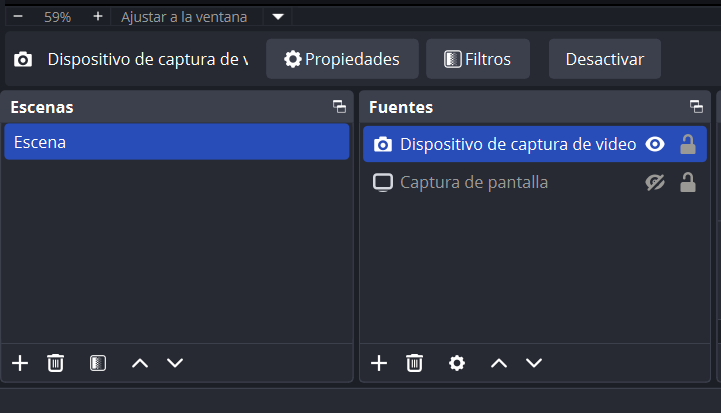
\includegraphics[width=0.9\textwidth]{Imagenes/Vectorial/filtroimagen.png}
    \caption{Ubicación en la interfaz de OBS Studio para el acceso al menú de filtros de una fuente.}
    \label{fig:filtro-imagen}
\end{figure}

Al seleccionar e incorporar el filtro, se desplegará la interfaz de configuración del plugin, confirmando la correcta vinculación del entorno de ejecución con las librerías dinámicas de visión computacional.

\section{Resolución de problemas }

En caso de que el filtro no aparezca listado dentro del menú de efectos de OBS Studio, se recomienda realizar las siguientes comprobaciones de diagnóstico:

\begin{itemize}
    \item \textbf{Verificación de rutas:} Revise minuciosamente que las librerías de OpenCV y Assimp se hayan copiado directamente en la raíz de \texttt{bin\textbackslash64bit\textbackslash} y no dentro de alguna subcarpeta accidental.
    \item \textbf{Integridad de versiones:} Confirme desde el menú \textit{Ayuda} $\rightarrow$ \textit{Acerca de OBS} que la versión instalada corresponde exactamente a la \texttt{31.1.1.2} de 64 bits. Las compilaciones de 32 bits no son capaces de cargar estas librerías.
    \item \textbf{Bloqueo de archivos:} Asegúrese de que el sistema operativo no haya bloqueado las librerías descargadas por motivos de seguridad. 
    \item \textbf{Inspección del Log del sistema:} OBS Studio registra de forma pormenorizada la carga de módulos durante el inicio. Acceda al menú superior \textit{Ayuda} $\rightarrow$ \textit{Archivos de registro} $\rightarrow$ \textit{Ver registro actual}. Busque líneas de error relacionadas con \texttt{obs-domjudge-ar-overlay.dll}. Si se muestra un error de tipo \textit{"LoadLibrary failed"}, esto indicará de manera inequívoca que falta alguna de las dependencias de OpenCV o Assimp en el directorio \texttt{bin\textbackslash64bit\textbackslash}.
\end{itemize}

\section{Proceso de desinstalación}

El plugin ha sido diseñado siguiendo una arquitectura modular limpia, por lo que no altera el registro del sistema de Windows ni genera ficheros residuales fuera de su entorno. Para realizar la desinstalación completa del software, siga estos pasos con la aplicación OBS Studio completamente cerrada:

\begin{enumerate}
    \item Acceda a la ruta \texttt{\textbackslash obs-studio\textbackslash obs-plugins\textbackslash 64bit\textbackslash} y elimine permanentemente el archivo \texttt{obs-domjudge-ar-overlay.dll}.
    \item Diríjase a la ruta \texttt{\textbackslash obs-studio\textbackslash bin\textbackslash 64bit\textbackslash} y elimine los siete archivos de dependencias previamente añadidos (\texttt{opencv\_*.dll} y \texttt{assimp-*.dll}).
\end{enumerate}

Una vez eliminados estos archivos, el sistema volverá a su estado original sin afectar el rendimiento o la configuración del resto de funciones de OBS Studio.